%%%%%%%%%%%%%%%%%%%%%%%%%%%%%%%%%%%%%%%%%%%%%%%%%%%%%%%%%%%%%%%%%%%%%%
% nuthesis-template.tex - Miguel A, Lerma - 3/31/2013
%                         mlerma@math.northwestern.edu
%%%%%%%%%%%%%%%%%%%%%%%%%%%%%%%%%%%%%%%%%%%%%%%%%%%%%%%%%%%%%%%%%%%%%%

%%%%%%%%%%%%%%%%%%%%%%%% DISCLAIMER %%%%%%%%%%%%%%%%%%%%%%%%%%%%%%%%%%
% 
% In spite of the effort to accommodate this template and the nuthesis
% class to the official requirements of the university to write a 
% Ph.D. dissertation, it is not possible to guarantee that it will 
% always work, and the author of the dissertation remains responsible
% for checking that such requirements are actually fulfilled by 
% his/her final work.
%
%%%%%%%%%%%%%%%%%%%%%%%%%%%%%%%%%%%%%%%%%%%%%%%%%%%%%%%%%%%%%%%%%%%%%%


\documentclass[12pt]{nuthesis}	% The nuthesis class is based on 
				% amsbook.cls.
				
\usepackage[english]{babel}
\usepackage[utf8x]{inputenc}
\usepackage[T1]{fontenc}
\usepackage[natbibapa]{apacite}
\usepackage{comment}
\usepackage{todonotes}
\usepackage{graphicx}


%%%%%%%%%%%%%%%%%%%%%%%%%%%%%%%%%%%
% DATA OF AUTHOR AND DISSERTATION %
%%%%%%%%%%%%%%%%%%%%%%%%%%%%%%%%%%%

\author{Matthew Heston}

\title{The Effect of Contextual and Relational Variables on Predicting Mobile Responsiveness}

%\degree{DOCTOR OF PHILOSOPHY}  % Default: DOCTOR OF PHILOSOPHY

\field{Technology and Social Behavior}            % Default: Mathematics

%\graduationmonth{June}         % The default is June or December
                                % depending on current date.

%\graduationyear{2003}          % Default: current year.


				% Use \includeonly to select the 
%\includeonly{chap1,chap2,...}	% chapters to include if you are 
				% using the \include command below.
				% This way you can latex only a the 
				% part you are working on, which 
				% is faster than latexing the entire 
				% thesis. 


\begin{document}
%	
%	THE BODY OF YOUR THESIS STARTS HERE
%

%%%%%%%%%%%%%%%%%%%%%%
% Some initial stuff %
%%%%%%%%%%%%%%%%%%%%%%

\frontmatter		% Preliminary pages start here.

\maketitle		% Produces the title page.

\copyrightpage		% Creates the copyright page.


\abstract		% Abstract.

This is the abstract.

\acknowledgements	% Acknowledgements (optional).

Text for acknowledgments.

\preface		% Preface (optional).

This is the preface.


%% A few more optional pages (uncomment if needed)
%
\listofabbreviations
CMC --- Computer Mediated Communication \\
SIP --- Social Information Processing Theory \\
SIA --- Session Initiation Attempt
%
%This is the list of abbreviations (optional).
%
%\glossary
%
%This is the glossary (optional).
%
%\nomenclature
%
%This is the nomenclature (optional).
%
%% Note that the dedication text must be passed as an argument
%% of the \dedication command
%\dedication{This is the dedication (optional).}
%

\clearpage\phantomsection % needed for the hyperlinks to work correctly
\tableofcontents	% Table of Contents will be automatically
			% generated and placed here.

\clearpage\phantomsection % needed for the hyperlinks to work correctly
\listoftables		% List of Tables and List of Figures will be placed

\clearpage\phantomsection % needed for the hyperlinks to work correctly
\listoffigures		% here, if applicable (optional).



\mainmatter             % Actual text starts here.

%%%%%%%%%%%%%%%%%%%%%%%%%%%
% Actual text starts here %
%%%%%%%%%%%%%%%%%%%%%%%%%%%

% If there is an introduction it must be the first chapter

\chapter{Introduction}

Responsiveness -- the amount of time it takes for a user to respond to a received message -- matters in computer-mediated communication (CMC). CMC users who violate expectations about responsiveness (e.g., who take too long to respond when a quick response is wanted) are often viewed more negatively than those who don't~\citep{cramton2002attribution,heston2017worth,kalman2011online} and communication scholars have suggested that users of CMC platforms use quick responsiveness to convey attributes like immediacy and presence~\citep{kalman2006pauses,walther1995nonverbal}. Given the importance of responsiveness in CMC, some empirical work on responsiveness has focused on what factors affect a user's decision to respond to an incoming message immediately or otherwise postpone their response~\citep{avrahami2008waiting,dabbish2005understanding}.

This decision to respond quickly or not is arguably more complicated with the growing use of mobile devices and mobile messaging platforms such as SMS. Most U.S. adults now own a mobile device~\citep{anderson2015technology} that they carry with them nearly constantly~\citep{oksman2003perhaps,rainie2015americans,turkle2008always}. Previous work on responsiveness focused on workplace CMC platforms such as email~\citep{dabbish2005understanding,tyler2003can} and instant messaging~\citep{avrahami2008waiting} on desktop computers,  where message senders could make some assumptions about the person they were trying to reach (e.g., that they were sitting at a desk on their computer during certain hours of the day). Mobile devices, on the other hand, have created a culture of perpetual contact~\citep{katz2002perpetual}, where device owners can be reached at any time and at any place, increasing the number of considerations when deciding to engage with an incoming message~\citep{avrahami2007improving,grandhi2010technology}.

We know, for example, that mobile messaging users are aware of normative expectations to be constantly available and feel pressure to respond quickly~\citep{church2013s}, which they also try to balance with their own desire to not be too dependent on their phones~\citep{ames2013managing,hall2012calling}. Users also report having different responsiveness behavior for different types of messages~\citep{cui2016beyond}, which is not surprising given that communicators adjust their conversational behavior based on the type of conversation they're having~\citep{levinson1981essential,sacks1974simplest}. We also know that mobile device owners use their devices to communicate with various types of contacts, including close friends, acquaintances, family, and co-workers~\citep{battestini2010large}. In face-to-face conversation, communicators change their behavior based on their relationship with their conversation partner~\citep{brown1987politeness,locher2005politeness}. We might also then expect mobile communicators to change responsiveness behavior based on their relationship with the person contacting them.

However, no work to date has focused on how much these various factors affect mobile responsiveness in a naturalistic setting. Qualitative work has helped to discover the many considerations users have in deciding when to respond~\citep[e.g.,][]{church2013s,cui2016beyond,wohn2015ambient}, but the magnitude of these effects remains unknown. Measuring these effects has important theoretical consequences.

Knowing how much these different factors affect responsiveness provides a better understanding of the discursive role of responsiveness in mobile CMC. Relatively large effects of relational variables, for example, would support the hypothesis that communicators use responsiveness to convey relational information~\citep{kalman2006pauses,walther1995nonverbal}, and indicate that responsiveness is similar to other communication behaviors that are relationally adjusted~\citep{locher2005politeness}. If, on the other hand, users simply respond to all of their contacts immediately, regardless of their relationship, it might indicate responsiveness should not be thought of in terms of a relationally dependent conversational behavior.

The extent to which different types of variables affect responsiveness is also useful for understanding how users navigate the tension between the benefits and drawbacks of the ``always on'' nature of mobile messaging. While being constantly reachable has allowed for new opportunities such as increased coordination~\citep{ling200210} and relational maintenance~\citep{pettegrew2015smart}, increased use of mobile devices for communication has also been associated with overdependence and decreased satisfaction in relationships~\citep{hall2012calling}. Users have reported using responsiveness strategically to signal availability and set expectations about mobile interaction (e.g., delaying response to decrease expectations for fast responses in the future)~\citep{ames2013managing,wohn2015ambient}. While responsiveness represents only one part of the larger questions about how phone owners deal with constant contact, it nevertheless is one useful measure to understand when users engage immediately with their device and when they are willing to postpone engagement.

Understanding what affects mobile responsiveness also has practical implications for the design of mobile text-based interaction platforms. HCI scholars have shown an interest in better supporting affective communication in mobile messaging platforms~\citep[e.g.][]{amin2005sensems}. With regards to responsiveness, recent work has suggested the design of awareness displays, showing a message sender the predicted likelihood of getting a response from the person they are trying to contact, thus mitigating the expectations of a fast response~\citep{pielot2014didn}. If a user's availability is the main factor affecting whether or not they will respond, this approach seems reasonable. If, however, message content greatly affects the decision to respond, these predictive systems may also need to explore understanding content to provide better predictions. If responsiveness is affected primarily by sender-receiver relationship, such a system likely lacks social nuance and would result in inaccurate predictions (e.g., a user may be available to respond, but choose not to because he does not consider the person reaching him to close enough to warrant an immediate response.)

The goal of this dissertation is to quantify the effects of availability, message content, and sender--receiver relationship on mobile responsiveness. Using SMS data and experience sampling data collected using a custom developed Android application from smart phone owners around the United States, the current work aims to contribute to our understanding of how these different factors affect responsiveness behavior in mobile messaging.

\chapter{Background}

\section{Cues in Computer-Mediated Communication}

Nonverbal communication is an essential part of how humans communicate, and includes a variety of elements such as appearance, touch, gaze, and proximity~\citep{burgoon2016nonverbal}. Nonverbal communication has been shown to be important in many areas, such as social influence and leadership skills~\citep{hogg2006social}, conflict resolution~\citep{ting2001managing}, and interpersonal attraction~\citep{burgoon1991relational,erceau2007tactile}.

The lack of these nonverbal cues was central to early theoretical approaches to CMC. Social Presence Theory~\citep{short1976social} described all media as fitting on a one-dimensional spectrum of \textit{social presence}, which refers to ``the degree of salience of the other person in an interaction''. Greater social presence was often tied directly to the nonverbal cues present in face-to-face (FtF) interaction~\citep[e.g.,][]{burgoon1984relational}, such that CMC, and especially text-based interaction, were thought to result in less social presence. It was also hypothesized that communicators would choose an appropriate medium for their message, e.g., avoid communicating potentially ambiguous message over a less rich medium given the higher likelihood of being misinterpreted~\citep{daft1986organizational}.

Such theories comprise what \citet{walther2002cues} refers to ``cues filtered out'' theories of CMC, so called because of their emphasis on the lack of nonverbal cues driving behavior. His own theory, Social Information Processing (SIP)~\citep{walther1992interpersonal}, rejects the notion that the lack of certain nonverbal cues restricts communicators' abilities. 

Conceptual models of social cognition in psychology described a ``social information processing'' system in which individuals decode various social stimuli about an interaction partner (e.g., physical traits and behaviors) over time to form a representation of the person~\citep{lord1985information}. This process was described as goal-motivated. \citet{wyer1980processing}, for example, discuss how the focus of information processing changes depending on whether you just want to get to know someone or are deciding to take them out to dinner. \citeauthor{walther1992interpersonal} applied this model to CMC, assuming that communicators have the same goals and motivations to form impressions of others in online environments. Rather than focusing on the lack of certain nonverbal cues or social stimuli such as physical traits, \citeauthor{walther1992interpersonal} noted that linguistic cues are also often used to convey relational information, such as form of address~\citep{argyle1976gaze} and other lexical choices~\citep{wiener1968language}. In addition to relying on these linguistic cues in CMC, he also noted the adoption of paralinguistic cues, such as emoticons, to convey emotion in CMC~\citep{carey1980paralanguage,sherblom1988direction}. In other words, whereas \citet{daft1986organizational} may suggest email is simply not appropriate for certain types of communication which may be thought of ambiguous, \citeauthor{walther1992interpersonal} would instead suggest email users adapt to the medium, encoding various cues to ensure a lack of ambiguity.

Early empirical work drawing on SIP focused on impression formation, i.e., individuals meeting each other in CMC environments and forming impressions over time~\citep[e.g.,][]{hancock2001impression,markey2002interpersonal,tanis2003social}. Nevertheless, as text-based communication platforms have become widely used not just for meeting others online, but for maintaining existing offline relationships~\citep{grinter2006chatting,pettegrew2015smart}, the same types of cues still are used to convey different types of information across different types of relationships~\citep{derks2008emoticons,pirzadeh2012expression}.

\subsection{Responsiveness}
SIP provides a useful conceptual framework to understand the role of responsiveness, or the time it takes for a communicator to respond to a message, in CMC. Timing has been demonstrated to be an important nonverbal element in FtF interaction~\citep{burgoon2016nonverbal}. \citet{mclaughlin1984conversation} details how different short gaps in conversation are a useful element of the turn-taking procedure, where speakers can interpret the gaps as a turn-allocation method. However, when a gap exceeds a certain limit, conversation partners may feel like conversation has broken down. In an experimental study, ~\citet{mclaughlin1982awkward} found that gaps of more than a few seconds led to conversation partners being rated as less competent conversationalists.

SIP posits that communicators are driven to refine their impressions of those they communicate with based on the cues available to them. In the same way that cues such as lexical choice~\citep{muir2017linguistic,nguyen2016effects} and emoticons~\citep{tossell2012longitudinal, walther2001impacts} have been shown to affect impressions, responsiveness in CMC has also been linked to impressions. In an experimental study, \citet{kalman2011online} found that long delays in email response led to lower evaluations of job candidates by managers. In another experiment, \citet{heston2017worth} found that relatively small delays in instant messaging resulted in lower social attraction among friends.

Knowing that their communication partners decode these cues, communicators are also motivated to use such cues strategically to convey information. Emoticons, for example, have been linked to the desire to convey sarcasm in CMC~\citep{wolf2000emotional}. Although studies such as \citet{kalman2011online} and \citet{heston2017worth} have shown an effect of how responsiveness is ``decoded'' (i.e., in affecting impressions), no work has studied the ``encoding'' process, in other words, if communicators deliberately alter responsiveness behavior in order to convey relational information. However, it has been hypothesized that communicators do use responsiveness to convey feelings of intimacy and closeness~\citep{kalman2006pauses,walther1995nonverbal}.

\section{Mobile Devices and Perpetual Contact}

The adoption of mobile devices has had wide-reaching effects on the way we communicate. Notably, it allows for what scholars have called \textit{perpetual contact}~\citep{katz2002perpetual}: given that individuals now carry their cell phones with them nearly constantly, they are able to be in contact with others nearly constantly. This has afforded many new opportunities. \citet{ling200210} noted mobile devices' enabling of \textit{micro-coordination}, the ability to, for example, immediately inform someone if you're running a few minutes late for a meeting. The increasing use of mobile messaging~\citep{duggan2015mobile,smith2015us} has allowed young phone owners to use these platforms for relational maintenance purposes, staying in touch with both close friends and acquaintances~\citep{pettegrew2015smart}.

Although these examples demonstrate the utility of mobile devices, perpetual contact has also been associated with less desirable outcomes. Constant contact has been reported to increased feelings of anxiety, as friends may become overdependent as a result of constantly checking in with one another~\citep{baym2015personal}. \citet{ames2013managing} discusses how constant contact can be overwhelming and how users sometimes turn off their devices or turn on ``airplane mode'' in order to be unreachable.

\citet{hall2012calling} refer to this as a ``duality of interdependence.'' ~\citet{baxter1993relationship} discuss how relationship satisfaction and relationship maintenance behaviors are affected by various dialectical tensions including an autonomy---connection contradiction. \citeauthor{hall2012calling} argue that this tension is inherent to the increased access afforded by mobile phone technology.

HCI scholars have explored various ways of easing this tension through the design of communication platforms. In an experimental study, \citet{avrahami2007improving} found that by providing contextual information to a message sender about a message receiver, the senders were able to better time their messages as to not interrupt the receivers at an inappropriate time. A similar approach was suggested by \citet{pielot2014didn}, who developed a machine learning model to infer a receiver's likelihood of engaging with a received message in order to inform a message sender of the receiver's current availability.

Other work suggests availability should be considered more malleable. In a field study of cell phone use, \citet{grandhi2010technology} found that who sent a message and what the content of the message were more important in the decision to engage with it than the user's current availability. Interview participants in a study by \citet{wohn2015ambient} also described content and sender--receiver relationship to be important factors in deciding when to respond to a message.

\subsection{Responsiveness}

The studies above demonstrate many interacting factors which should affect responsiveness behavior in mobile messaging. \citet{bayer2015connection} argue that increased use of mobile devices has resulted in new normative expectations about constant connectivity. There is some empirical support for this proposition in \citet{church2013s}, whose interview participants reported expecting immediate response from those they contact on mobile messaging. This perspective does not contradict SIP --- users may still encode relational information through their responsiveness behavior --- but it does suggest that users' behavior may also be affected by these new expectations.

At the same time, interview participants across studies have expressed frustration with these expectations~\citep{ames2013managing}, and reported that relational and contextual factors are still the primary factors which affect their responsiveness behavior~\citep{grandhi2010technology,wohn2015ambient}. These findings suggest that while users may be aware of expectations for fast responsiveness on mobile devices, they prioritize messages and decide whether or not to respond immediately, basing their decision on factors such as message content and who is trying to reach them.

\section{Relational Work in Communication}

Several of the above studies suggest that sender--receiver relational attributes should affect responsiveness behavior~\citep[e.g.,][]{grandhi2010technology,kalman2006pauses,walther1995nonverbal,wohn2015ambient}, but it is not always clear what relational attributes are associated with responsiveness behavior and how they can be measured. If we assume responsiveness is serving a discursive function in text-based interaction, it is useful to consider work in conversation analysis and sociolinguistics that describes various relational attributes and how they affect conversation dynamics.

\citet{sacks1974simplest} conceptualized of conversation as a series of ``turn-taking units,'' wherein conversation partners follow a set of accepted procedures in responding to one another. Central to this model of conversation is the notion that each utterance serves a specific function, and understanding this function is what allows the responding partner to reply appropriately. \citet{levinson1981essential} critiqued this model, suggesting that constraints in conversation are strategy based rather than rule based. In other words, a conversation participant does not choose how to respond solely based on the function of the preceding utterance, but based on his interactional goals. Consider, for example, a phone call between two friends where one friend is running late for dinner. The late friend might begin the conversation with a greeting (``Hello?''). Whereas a rule-based model of conversation may predict the second party to respond with a greeting, as that is typical in conversations, a strategy-based model may predict skipping the greeting in order to display frustration about running late (``Where are you?'').

This strategic approach is present the development of ``facework'' by \citet{brown1987politeness}, who suggest that interactants mutually adapt their conversational behavior to avoid embarrassment of one another. While \citeauthor{brown1987politeness} discuss their theory in terms of politeness behavior, \citet{locher2005politeness} suggest the theory applies more broadly to negotiating what is appropriate or inappropriate behavior, referring to the ``work'' involved in this negotiation as \textit{relational work}.

If responsiveness is driven in part by norms and expectations ~\citep[e.g.,][]{bayer2015connection, church2013s}, relational work provides a useful theoretical frame to understand how that behavior is adapted across relational contexts. \citet{brown1987politeness} suggest two primary relational dimensions that should affect relational work decisions: closeness and power, where closeness refers to the degree of friendship between actors and power refers to any status difference between them. These are also the primary relational attributes discussed by \citet{spencer2011conceptualising} in her review of interpersonal pragmatics.

The effect of these relational attributes on conversational behaviors has been observed in various contexts. In an experimental study, intimacy was significantly associated with the choice of relational work strategies~\citep{meyer2004repairing}. In observational studies of the workplace, where hierarchical status differences make power differentials more clearly defined, differences in power have been shown to affect behaviors such as requests and directives~\citep{craven2010directives,vine2009directives} . With regard to CMC, and in particular mobile messaging, a discourse analysis of SMS messages by \citet{laursen2005please} noted closeness as directly impacting response norms, with similar discursive studies finding closeness affects other normative behaviors in SMS, such as how users choose to end interactions~\citep{spilioti2011beyond}.

\chapter{The Current Project}

Responsiveness may be seen as a cue in the Social Information Processing theory of CMC. CMC scholars have suggested that fast responsiveness may be associated with immediacy and care in CMC \citep{kalman2006pauses,walther1995nonverbal}, and experimental studies have demonstrated that slow responsiveness across different text-based platforms can lead to negative evaluations~\citep{heston2017worth,kalman2011online}.

However, most cues that have been studied from a SIP perspective are explicitly encoded by a sender. Studies such as ~\citet{hancock2007expressing} and ~\citet{pirzadeh2012expression} focus on cues such as word choice, punctuation, and emoticons, all of which a message sender can choose to alter when writing a message. Responsiveness, on the other hand, may not always be a conscious choice, as an individual may not respond simply because he is busy. Responsiveness is affected by many different factors.

The first is likely simply the message receiver's availability. In addition to simply not having access to their device, ~\citet{avrahami2007improving} noted various situational factors that could affect a cell phone owner's decision to take a call, such as if they were currently with a group and would be soon as rude for leaving to accept the call. Even now as social norms shift and being on a phone to respond to a message may seem less inappropriate~\citep{rainie2015americans}, individual users likely have their own set of guidelines that govern a subjective sense of being available for incoming mobile messages.

If availability were the primary factor driving responsiveness behavior, responsiveness would represent a unique type of cue from a SIP perspective: one that is ``encoded'' almost entirely by external forces, but that nevertheless is decoded in a way that affects impressions of a conversation partner in CMC. Investigating the relationship between availability and responsiveness also provides a baseline to compare how important other factors are in affecting responsiveness. My first research question then is:

\textit{RQ1: What is the relationship between a user's current availability and their mobile responsiveness?}

Other factors may also affect responsiveness, however. From a turn-taking perspective of conversation~\citep{sacks1974simplest}, a participant in a conversation will know how to use his turn based on various cues from the previous turn. In mobile messaging, a user might decide to respond quickly based on certain attributes of a received message. For example, someone might be busy and not want to get involved in a text conversation, but nevertheless choose to respond right away to an request for information from someone, under the assumption that that will be the end of their exchange. Furthermore, certain cues in CMC have been associated with heightened urgency or immediacy~\citep{nguyen2014lexical}, which may cause a message receiver to respond more quickly. These effects may ``override'' a user's current availability, assuming they are available enough to see the message.

If these effects were strong, responsiveness more closely resembles the type of cues hypothesized by scholars such as ~\citet{walther1995nonverbal} and ~\citet{kalman2006pauses}, where the responsiveness behavior more closely resembles a deliberate choice made by a conversation participant in response to cues they perceive in a received message. My second research question is:

\textit{RQ2: What is the relationship between attributes of an incoming message, such as perceived urgency, and responsiveness? Is this relationship affected by a user's current availability?}

Finally, the relationship between a message sender and receiver could also affect responsiveness decisions. Work within social pragmatics has suggested various relational attributes that affect the conversation dynamics between parties~\citep{brown1987politeness,goldberg1990interrupting,west1979against,wolfson1990bulge}, and qualitative studies of mobile messaging have suggested social pressure can affect responsiveness behavior~\citep{church2013s}. In particular, the degree closeness between individuals, sometimes referred to as intimacy, along with status differences between individuals have been empirically shown to affect various nonverbal communication behaviors~\citep{guerrero1991waxing,henley1973power,leffler1982effects,sternglanz2004reading}.  At the same time, recent work has argued certain social pragmatic behavior that exists FtF is less important in CMC~\citep{schulze2017knowledge,stromer2015context}, so the relational attributes previously focused on by conversation analysts may not be as important in CMC, at least with regard to responsiveness decisions. In the same way as message-level attributes may ``override'' situational factors, the same may occur with these relational variables, i.e., a user may respond quickly to his boss even if he is busy because he feels pressure to seem available given their relationship.

Quantifying the effect of relational variables on responsiveness behavior will both allow us to see if the same relational attributes demonstrated to affect conversation behavior FtF also exists in CMC, as well as understand how responsiveness as a cue might vary based on relationship, building on work that has studied how other SIP cues change based on relational context~\citep[e.g.,][]{hancock2007expressing}. My final research question is:

\textit{RQ3: How do intimacy and status between a message sender and message receiver affect responsiveness? Is this effect affected by a user's current availability?}


\chapter{Methods}

\section{Participants}

Participants were recruited online using Craigslist ads, Facebook ads, and Reddit posts. Ads were posted in the 10 most populous US cities. Participants were required to be at least 18 years old, native English speakers, and own an Android phone running at least version 6.0 of the Android OS~\footnote{At the time the study was run, Android 6.0 was the minimum OS version still being actively supported.}. Participants were compensated with a \$20 Amazon gift card in exchange for participation in the study. A total of 233 participants took the initial survey. Of those participants, 126 installed the Android application. Of those that installed the application, 93 completed the entire study. All analysis results refer to these 93 participants that completed the study procedure.

Gender was slightly skewed with 58\% female participants. A majority of participants were Caucasian (72\%), while 15\% were Black / African American, 13\% were Asian, and 4\% were American Indian. One participant preferred not to disclose ethnicity. Participant age ranged from 18 to 71 years old, with a median age of 30 years old. Age distribution is shown in Figure~\ref{fig:age}.

\begin{figure}[h]
\centering
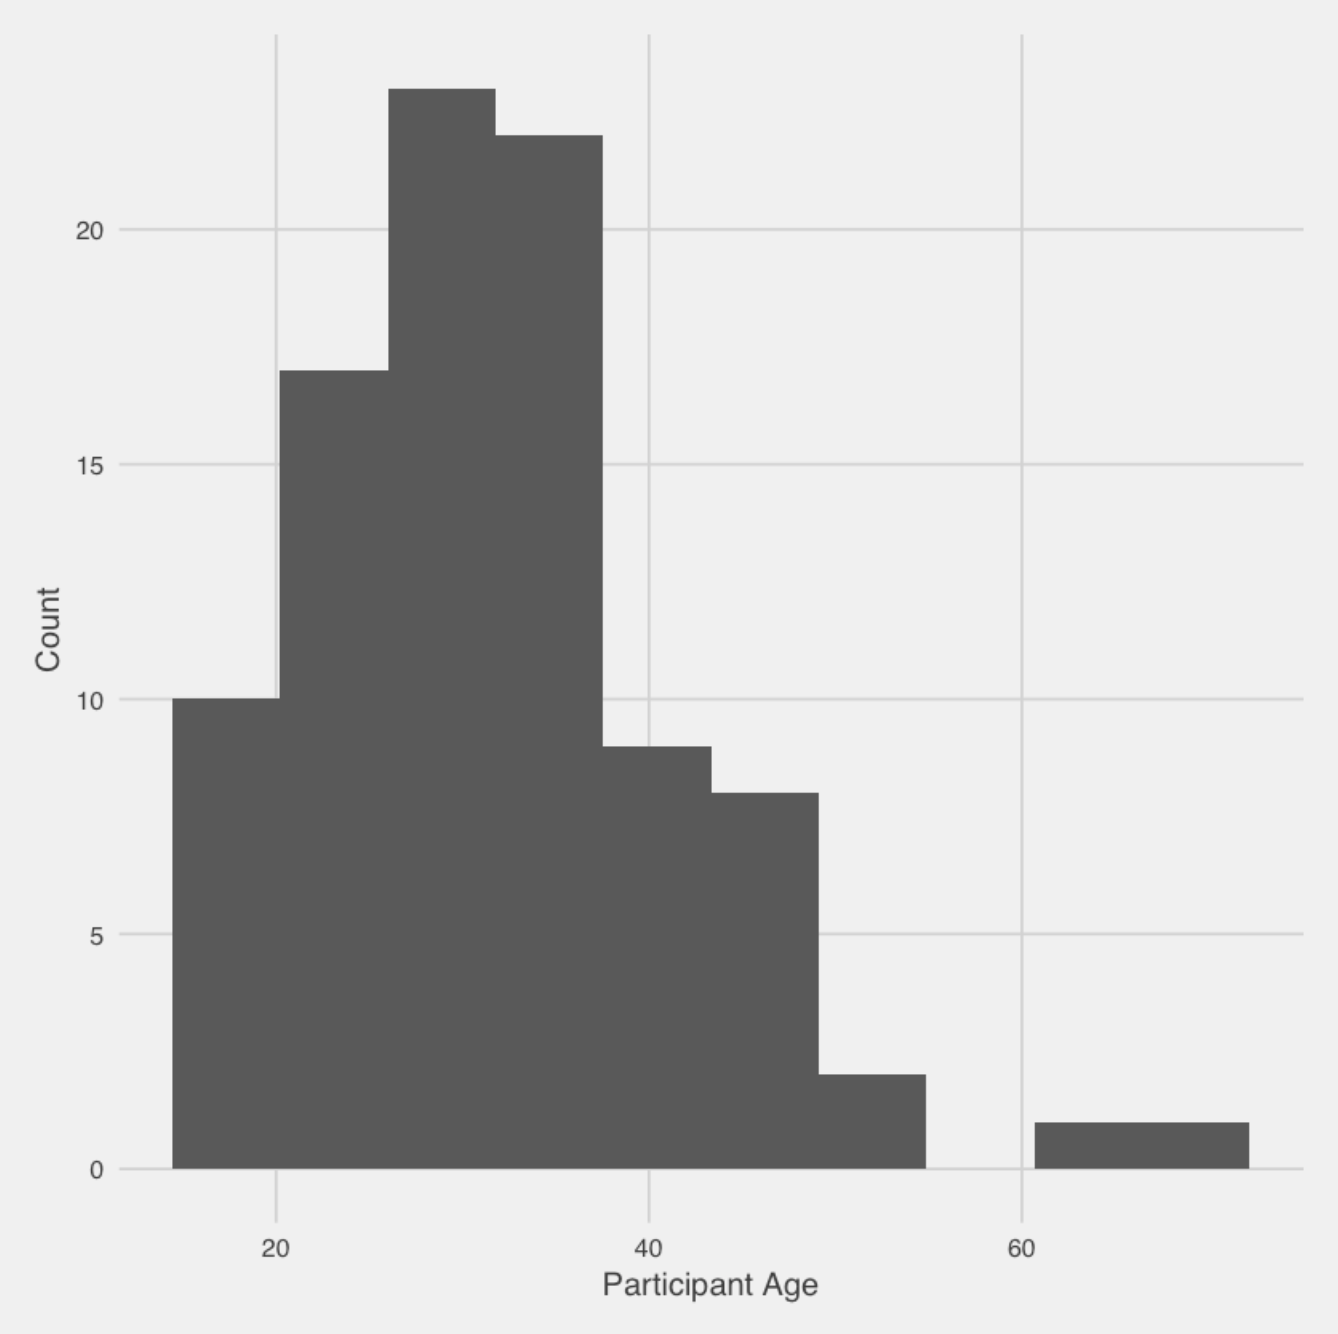
\includegraphics[width=.7\textwidth]{figures/age_distribution}
\caption{Distribution of participant ages}
\label{fig:age}
\end{figure}


\section{Procedure}

\subsection{Pre-Study Survey}

Recruitment materials directed participants to an initial survey, which was used to collect the demographic information reported above, information about how participants used their phones, as well as a personality assessment.

\subsubsection{Texting Use}
Given that restrictions on texting, such as having a limited text plan, could influence the texting behavior of interest in the study, participants were asked if they were aware of any limits on their SMS plan. No participants reported having such limits.

While the focus of this study is on SMS, other messaging platforms such as Google Hangouts and Facebook Messenger are also popular. Participants were asked what other messaging applications they use, and how their use of SMS compared to the use of these other platforms. All participants reported using at least one other messaging application. Forty-six percent of participants said they used SMS more often than these other applications, and 28\% reported using SMS about the same amount as the other applications. Twenty-five percent said they use SMS somewhat less often than other messaging applications, with only 1\% reporting using SMS a lot less often.

%\subsubsection{Personality Data}
%Prior work has demonstrated a link between the ``Big 5'' personality traits~\citep{john1991big} and various mobile phone behaviors, including frequency of SMS use as well as responsiveness to SMS messages~\citep{chittaranjan2011s,de2013predicting,lepp2015exploring}, suggesting these traits may be a useful covariate to include in a responsiveness model. These traits were measured using a modified short version of the scale developed by \citet{rammstedt2007measuring}.
%\todo[inline]{Put texting info here.}

\subsection{SMS Tracking Application}

After completing the pre-study survey, participants were emailed a link to a custom Android application developed to collect their text messages and experience sampling data when responding to messages. They were also provided with detailed instructions about the app and measures involved. Participants were required to run the app for 7 days. No data after 7 days was collected.

A background service monitored participants' SMS database, storing all messages sent and received during the study period on an external database, managed by Northwestern School of Communication IT. All sensitive information, including phone numbers and message content, were encrypted before being sent to the database. These encrypted values were also stored in the database to help ensure participant privacy. Multimedia content, such as photographs, were not stored. Only dyadic conversations were stored (i.e., not group texts).

\subsubsection{Session Initiation Attempts}

The focus of this study is on responses to what \citet{avrahami2006responsiveness} call \textit{session initiation attempts} (SIA's). An SIA is any message that begins a new conversation session. Once users are engaged in a texting conversation, they tend to respond quickly~\citep{battestini2010large}, whereas we would expect more variation in responsiveness in deciding whether or not to engage with a conversation initiation.

SIA's were identified using a heuristic similar to \citet{avrahami2006responsiveness}, where an SIA is any incoming message from a contact that is sent after some threshold has passed since the last received message from that contact. The threshold chosen for this study was 30 minutes, which was selected after reviewing large scale studies of texting behavior~\citep{battestini2010large,birnholtz2017attending}, as well as discussion with pilot study participants. To illustrate SIA's, note that in Figure~\ref{fig:sia} the incoming message that starts ``Hey, I don't want to wait...'' would be considered an SIA since days have passed since the last interaction, as would ``So like 1 or 2'' since it has been more than 30 minutes since the last message the ``What time do you want to leave?'' message was sent, whereas the ``ok'' emoji would not, since only 11 minutes have passed.

%A potential issue with this heuristic approach is that it ignores ``follow up'' texts. Imagine, for example, that the session initiator in Figure~\ref{fig:sia} followed up their 12:56pm ``What time do you want to leave'' text with a 1:00pm text that just said ``??'', a technique that has been observed to heighten attention from a contact~\citep{heston2017worth}. In this case, we are still interested in responsiveness as it related to the initial 12:56pm text. To deal with this, if a message was registered as an SIA, any follow up texts sent during the next half hour were grouped with that initial text.

\begin{figure}[h]
\centering
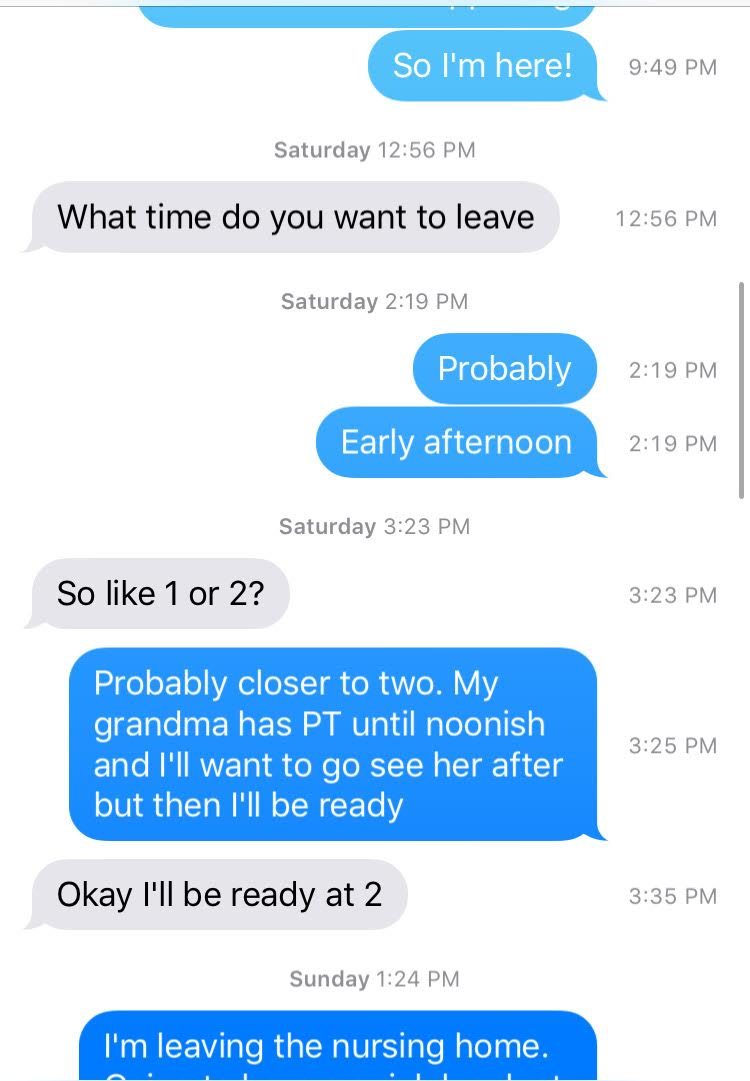
\includegraphics[width=.7\textwidth]{figures/example_sia}
\caption{Example text message exchange}
\label{fig:sia}
\end{figure}


\subsection{Experience Sampling}

Whenever a participant responded to an SIA, they would receive a notification on their phone to fill out a short questionnaire about the message they were responding to, following an event-based approach to experience sampling~\citep{conner2009experience,csikszentmihalyi2014validity}. It is normally recommended experience sampling  be triggered immediately at the moment of interest~\citep{hormuth1986sampling}, e.g., in this case, participants could be asked about text message the moment it is received, rather than when they respond to it, removing the need for a retrospective answer. However, this could have other consequences which affect study validity. Our primary variable of interest is response time. Sending the user multiple notifications about an incoming message (i.e., both the notification for a message and the notification asking for their availability), could cause the participant to behave differently than they otherwise would, e.g., responding to the message when they otherwise wouldn't, since they are responding to our prompt anyway.

When taken to the questionnaire, participants were shown the message they just sent, the contact they sent it to, the initial SIA they were responding to, and the time that SIA was received. They were then asked to rate the following items:

\textbf{Availability.} Participants were asked to rate their availability in 2 ways. The first involve a dichotomous ``unavailable'' measure. Participants could make themselves as totally unavailable in the case of having left their phone at home, their phone being in their backpack, or any situation in which they could not reasonable access their phone at all.

If a participant was not totally unavailable, they were asked to rate their availability on a scale of 1--5, with 1 indicating being very busy or otherwise distracted, and 5 representing being not busy at all.  A similar single item scale was used to assess availability in ~\citet{fogarty2005predicting}.

Other responsiveness studies have used sensor data, such as phone activity, to make inferences about availability, rather than using experience sampling to collect this directly~\citep[e.g.,][]{pielot2014didn}. However, such studies focus only on predicting responsiveness, rather than explaining responsiveness behavior. Given the focus of this work on understanding how different variables affect responsiveness, capturing an availability measure directly should allow for better inference in how message content and sender-receiver relationship interact with a participant's own subjective feeling of availability.

\textbf{Message Importance.} In studies of other CMC platforms, such as email, the perceived importance of a received message affects how users prioritize messages~\citep{siu2006going,tsugawa2012estimating} and messages thought to be more important receive quicker responses~\citep{dabbish2005understanding,wainer2011should}. Participants rated each SIA on a two 1--5 scales, ``How important is this message to you?'' and ``How important do you think this message is to the person who sent it to you?''


\subsection{Post-Study Survey}

After running the SMS tracking application for 7 days, participants were sent a final survey where they rated each of their contacts who sent them an SIA during the study on 2 relational scales. Intimacy was measured using a 3 item scale adapted from \citet{miller1982assessment}. Power was measured using a 3 item scale adapted from \citet{farrell2015relationship}. The distribution of these variables across contacts are shown in Figures \ref{fig:intimacy} and \ref{fig:power}. To account for potential differences in texting behavior based on the proximity of the message sender to the message receiver (e.g., a person may have different texting habits with someone who lives in their same city that they see often versus a friend who lives in a different state who they see rarely), for each contact, participants also specified proximity from one of the following options: ``We live together,'' ``In the same city, but we don't live together,'' ``In the same state, but not the same city,'' ``In the same timezone, but not the same state,'' ''In a different time zone.''


\begin{figure}[h]
\centering
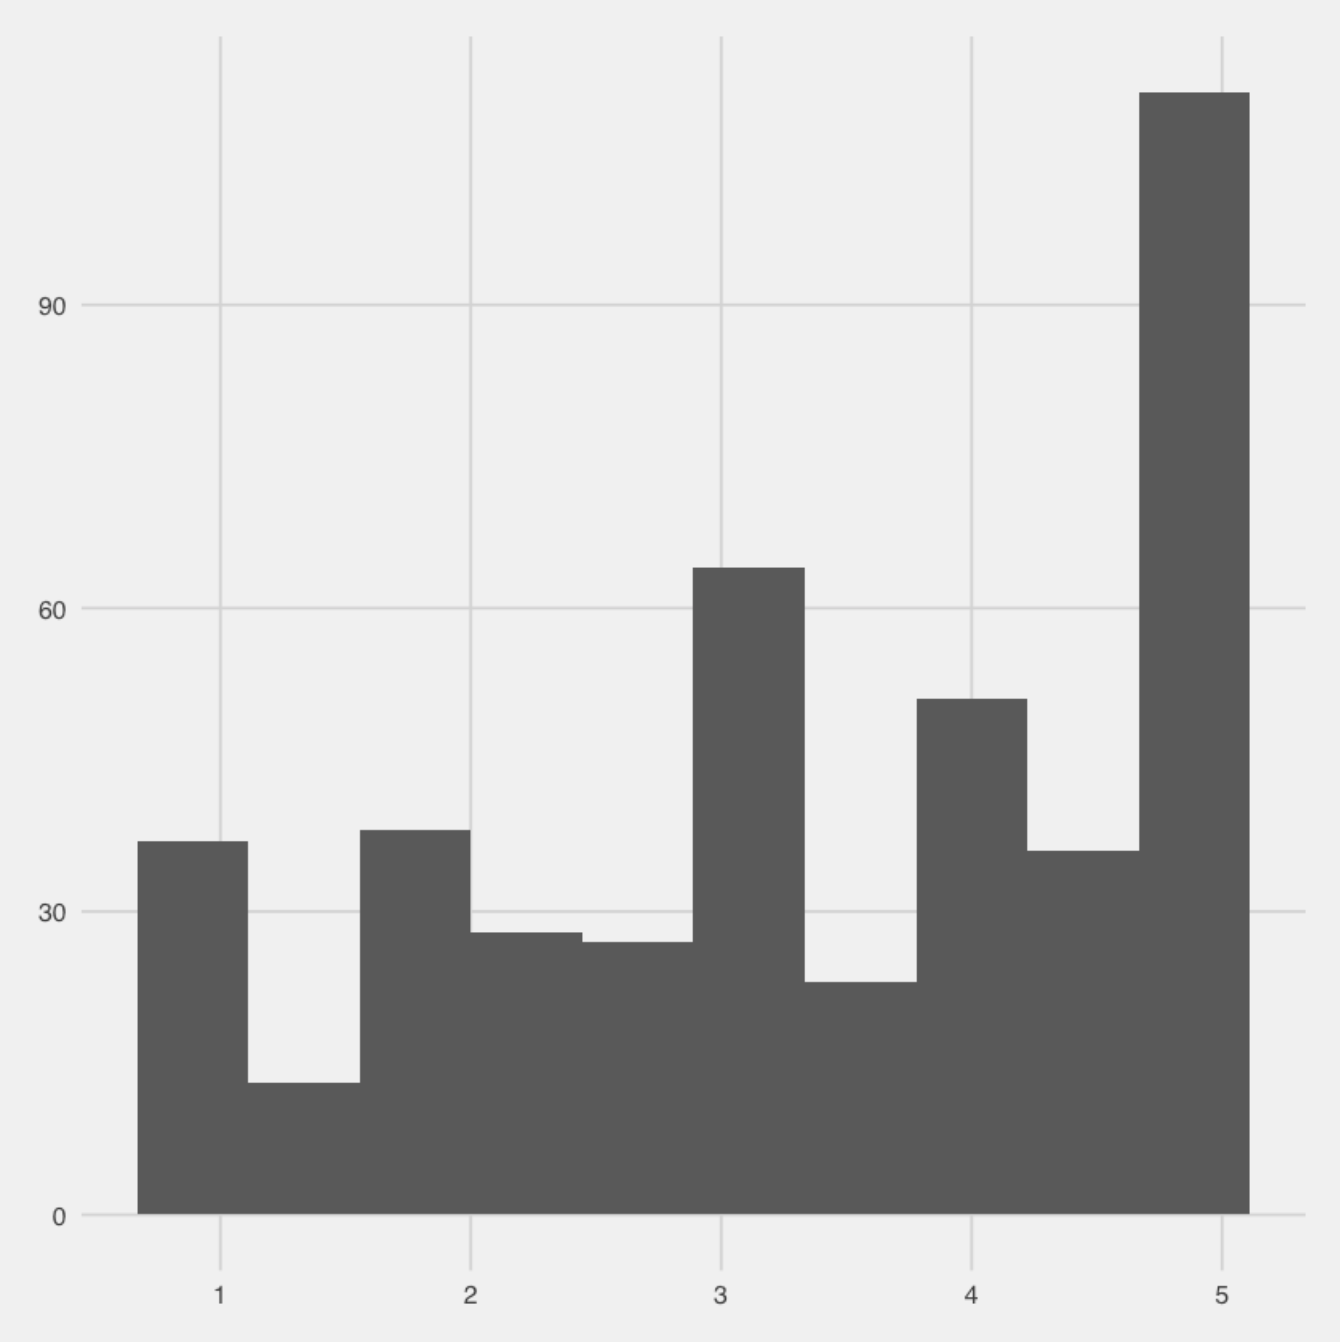
\includegraphics[width=.7\textwidth]{figures/intimacy_distribution}
\caption{Distribution of measured intimacy across contacts.}
\label{fig:intimacy}
\end{figure}


\begin{figure}[h]
\centering
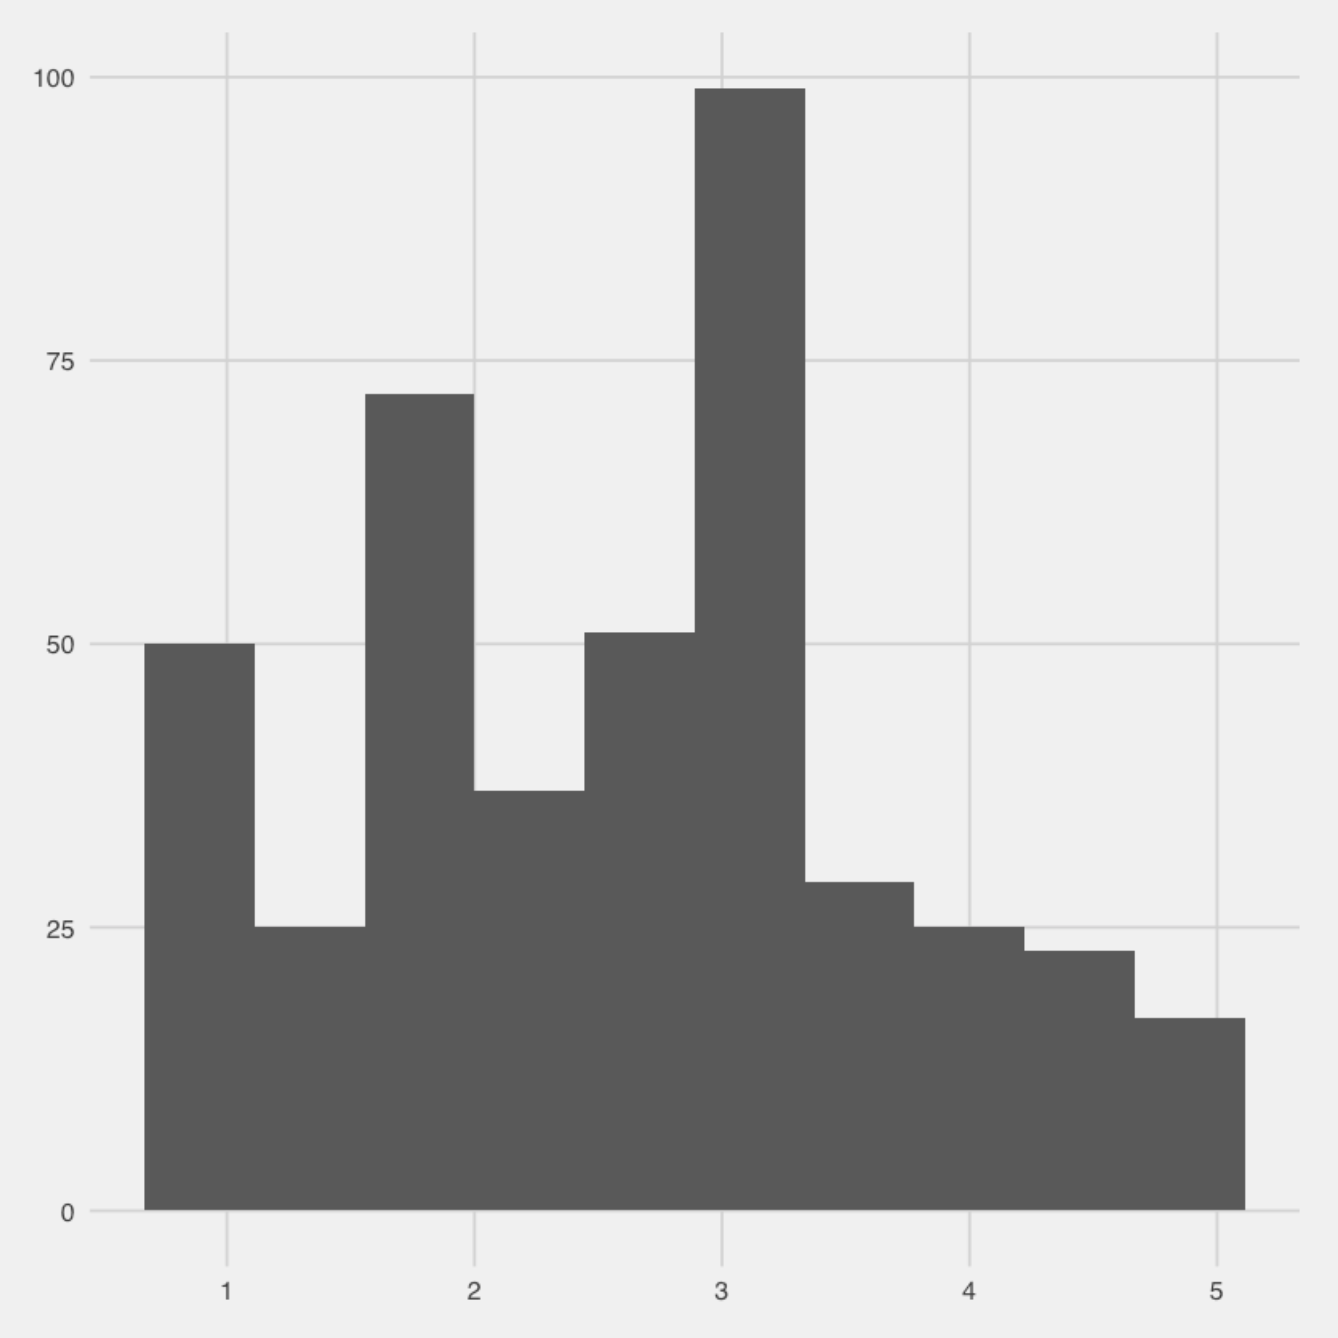
\includegraphics[width=.7\textwidth]{figures/power_distribution}
\caption{Distribution of measured power across contacts.}
\label{fig:power}
\end{figure}

\subsection{Post-Study Content Coding}

Requests for information or action have been shown to increase the likelihood of engaging with a message~\citep{dabbish2005understanding}. After data collection was completed, content coding was performed on SIA's to categorize them as either being a request or not.

\section{Analysis}

Given the hierarchical nature of the collected data (e.g., SIA's are grouped within contacts which are grouped within participants), data was analyzed using a series of multi-level models~\citep{gelman2007data}.

In all regression models, the dependent variable was the natural log of the seconds in response latency between the receipt of an SIA and the response. The distribution of response time in seconds, shown in Figure~\ref{fig:response_time}, is highly skewed, which is typical of response time distributions~\citep{kalman2006pauses}. Taking the log of this variable results in a more normal distribution, as shown in Figure~\ref{fig:log_response_time}. Other approaches to dealing with this type of skewed data include different classes of generalized linear models~\citep[see e.g.,][]{buntin2004too,dick2004beyond,manning2001estimating}, but experimentation with these models demonstrated poor model fit for the collected data.

To understand the impact of how different classes of independent variables (i.e., contextual variables and relational variables) affect responsiveness, a hierarchical regression process was followed wherein a series of regression models were fit introducing a new class of variables at each step~\citep{gurnsey2017statistics}. To test whether or not variables improved model fit, likelihood ratio tests were used to compare models. In addition to these tests, model fit parameters such as the Akaike information criterion (AIC) were compared, as suggested by \citet{gelman2007data}.

\begin{figure}[h]
\centering
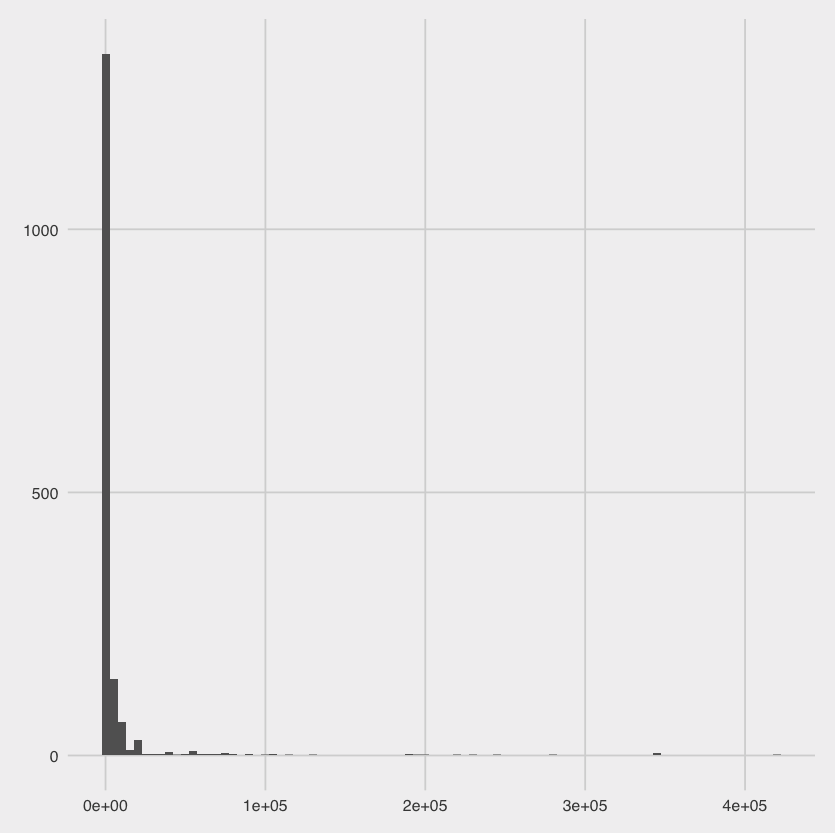
\includegraphics[width=.7\textwidth]{figures/response_time_distribution}
\caption{Distribution of response time in seconds.}
\label{fig:response_time}
\end{figure}

\begin{figure}[h]
\centering
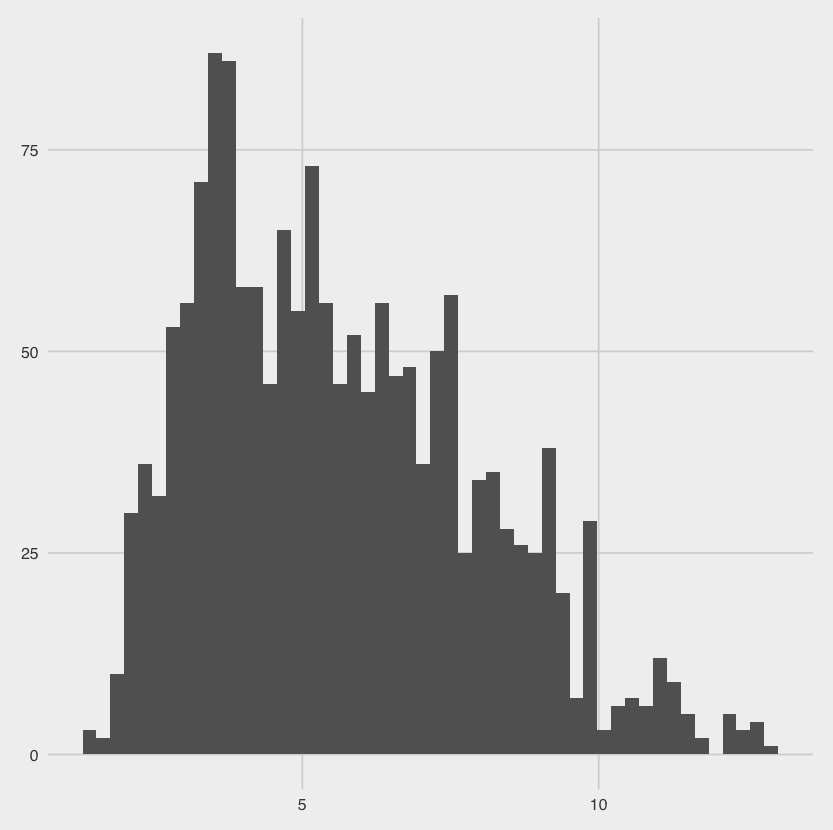
\includegraphics[width=.7\textwidth]{figures/log_response_time_distribution}
\caption{Distribution of the natural log of response time in seconds.}
\label{fig:log_response_time}
\end{figure}

\section{Results}

\subsection{Regression Results}

% Table created by stargazer v.5.2 by Marek Hlavac, Harvard University. E-mail: hlavac at fas.harvard.edu
% Date and time: Thu, May 10, 2018 - 17:38:33
\begin{table}[!htbp] \fontsize{7}{7.5}\selectfont \centering 
\begin{tabular}{@{\extracolsep{5pt}}lcccc} 
\\[-1.8ex]\hline 
\hline \\[-1.8ex] 
 & \multicolumn{4}{c}{\textit{Dependent variable:}} \\ 
\cline{2-5} 
\\[-1.8ex] & \multicolumn{4}{c}{log(response\_delay)} \\ 
\\[-1.8ex] & (1) & (2) & (3) & (4)\\ 
\hline \\[-1.8ex] 
 age & 0.005 & 0.004 & 0.004 & 0.005 \\ 
  & (0.017) & (0.017) & (0.017) & (0.017) \\ 
  & & & & \\ 
 genderMale & $-$0.210 & $-$0.286 & $-$0.329 & $-$0.326 \\ 
  & (0.287) & (0.294) & (0.295) & (0.292) \\ 
  & & & & \\ 
 sent\_total & $-$0.089 & $-$0.104 & $-$0.129 & $-$0.128 \\ 
  & (0.112) & (0.114) & (0.115) & (0.114) \\ 
  & & & & \\ 
 availability & $-$0.497$^{***}$ & $-$0.500$^{***}$ & $-$0.499$^{***}$ & $-$0.549$^{***}$ \\ 
  & (0.032) & (0.032) & (0.032) & (0.070) \\ 
  & & & & \\ 
 importance &  & $-$0.167$^{***}$ & $-$0.173$^{***}$ & $-$0.108$^{*}$ \\ 
  &  & (0.054) & (0.054) & (0.059) \\ 
  & & & & \\ 
 importance\_to\_contact &  & 0.069 & 0.072 & 0.009 \\ 
  &  & (0.055) & (0.055) & (0.060) \\ 
  & & & & \\ 
 requestar &  & 1.512$^{***}$ & 1.511$^{***}$ & 1.246$^{***}$ \\ 
  &  & (0.207) & (0.207) & (0.231) \\ 
  & & & & \\ 
 requestir &  & $-$0.010 & $-$0.021 & $-$0.016 \\ 
  &  & (0.125) & (0.125) & (0.133) \\ 
  & & & & \\ 
 power &  &  & 0.182 & 0.207 \\ 
  &  &  & (0.125) & (0.128) \\ 
  & & & & \\ 
 intimacy &  &  & $-$0.049 & $-$0.061 \\ 
  &  &  & (0.099) & (0.101) \\ 
  & & & & \\ 
 distance\_factorDifferent Timezone &  &  & $-$0.041 & $-$0.082 \\ 
  &  &  & (0.331) & (0.330) \\ 
  & & & & \\ 
 distance\_factorLive Together &  &  & $-$0.551$^{**}$ & $-$0.532$^{*}$ \\ 
  &  &  & (0.279) & (0.278) \\ 
  & & & & \\ 
 distance\_factorSame State &  &  & 0.064 & 0.063 \\ 
  &  &  & (0.222) & (0.222) \\ 
  & & & & \\ 
 distance\_factorSame Timezone &  &  & $-$0.243 & $-$0.291 \\ 
  &  &  & (0.382) & (0.381) \\ 
  & & & & \\ 
 availability:importance &  &  &  & $-$0.069$^{**}$ \\ 
  &  &  &  & (0.030) \\ 
  & & & & \\ 
 availability:importance\_to\_contact &  &  &  & 0.087$^{***}$ \\ 
  &  &  &  & (0.030) \\ 
  & & & & \\ 
 availability:requestar &  &  &  & 0.319$^{***}$ \\ 
  &  &  &  & (0.123) \\ 
  & & & & \\ 
 availability:requestir &  &  &  & $-$0.007 \\ 
  &  &  &  & (0.071) \\ 
  & & & & \\ 
 availability:power &  &  &  & $-$0.024 \\ 
  &  &  &  & (0.041) \\ 
  & & & & \\ 
 availability:intimacy &  &  &  & 0.007 \\ 
  &  &  &  & (0.035) \\ 
  & & & & \\ 
 Constant & 6.601$^{***}$ & 6.735$^{***}$ & 6.925$^{***}$ & 6.948$^{***}$ \\ 
  & (0.530) & (0.548) & (0.567) & (0.564) \\ 
  & & & & \\ 
\hline \\[-1.8ex] 
Observations & 1,635 & 1,635 & 1,635 & 1,635 \\ 
Log Likelihood & $-$3,347.506 & $-$3,320.159 & $-$3,321.296 & $-$3,325.114 \\ 
Akaike Inf. Crit. & 6,711.012 & 6,664.319 & 6,678.592 & 6,698.228 \\ 
Bayesian Inf. Crit. & 6,754.207 & 6,729.112 & 6,775.781 & 6,827.813 \\ 
\hline 
\hline \\[-1.8ex] 
\textit{Note:}  & \multicolumn{4}{r}{$^{*}$p$<$0.1; $^{**}$p$<$0.05; $^{***}$p$<$0.01} \\ 
\end{tabular} 
  \caption{Fixed Effect Estimates} 
  \label{tab:fixed_effects} 
\end{table} 

Estimated fixed effects from regression models are shown in Table~\ref{tab:fixed_effects}. All models included age and gender as covariates. In order to control for the texting activity, the log of the number of texts a participant sent over the 1 week study period was also included as a covariate. Model 1 included these control variables as well as the 0-5 availability measure. Model 2 introduced the message content variables importance, importance to contact, and if the message was a request. Model 3 included the relational variables intimacy, power, as well as propinquity. Model 4 included interactions between message content and relational variables and availability.

\subsubsection{Availability}

\textit{RQ1} asked what is the relationship between a user's current availability and their mobile responsiveness. As seen in Table~\ref{tab:fixed_effects}, the availability variable has a large, significant effect on predicting mobile responsiveness.  A unit increase on the 0-5 availability scale is associated with a decrease in response time in seconds by approximately 40\%.

\subsubsection{Message Attributes}

\textit{RQ2} asked about the relationship between message attributes and mobile responsiveness to that message. Model 2, which introduced these message attribute variables, significantly improved model fit over Model 1 which only included responsiveness ($\chi^2(4) = 66.64$, p < .001). Participants rated messages on 1-5 scales on how important a message was to them and how important they believe the message was to the contact who sent it to them. A unit increase on the importance to participant scale is associated with a significant 15\% decrease in responsiveness. The effect of the importance to contact variable was small and insignificant.

Messages were coded as not a request, an information request, or an action request. Information requests did not differ significantly from non-requests. On the other hand, responses to action requests took approximately 4.5 times longer than responses to non-requests.


\subsubsection{Relational Variables}

\textit{RQ3} asked about how message sender--receiver relationship affects mobile responsiveness. Model 3 introduced the power, intimacy, and propinquity variables. Power and intimacy are continuous variables measured on a 5 point scale and propinquity is a factor.

These variables did not significantly improve model fit ($\chi^2(6) = 6.46$, p = .37). Responses to a contact that a participant lived with were significantly 40\% faster than to contacts who only lived in the same city as the participant, but neither power or intimacy had significant effects on responsiveness.

\subsubsection{How Message Attributes and Relational Variables}

Both \textit{RQ2} and \textit{RQ3} asked how message attributes and relational variables moderate the effect of availability on mobile responsiveness. Model 4 included interaction terms between message attribute and relational variables with availability.

The inclusion of these interaction terms significantly improved model fit ($\chi^2(10) = 21.00$, p = .02). Significant interactions with availability were found for both importance measures as well as action requests. Figures~\ref{fig:importance_availability_interaction},~\ref{fig:importance_contact_availability_interaction}, and \ref{fig:request_availability_interaction} display predicted values from Model 4 to visualize these interactions.

\begin{figure}[h]
\centering
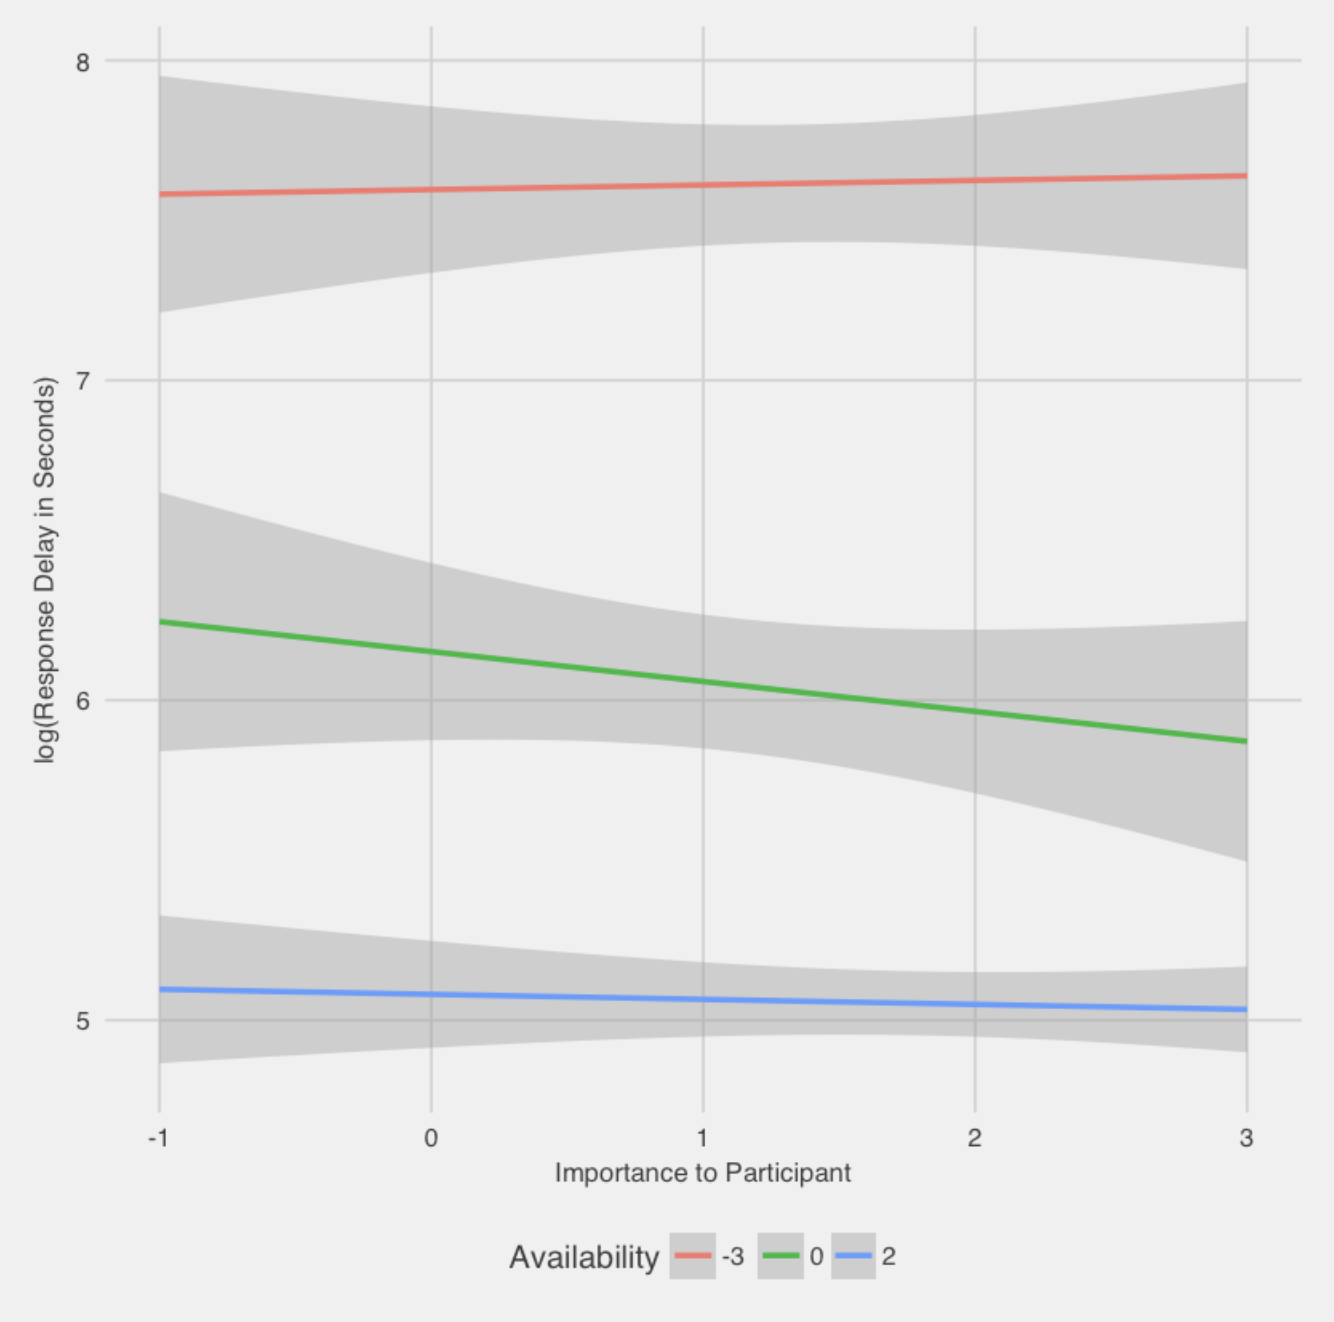
\includegraphics[width=.7\textwidth]{figures/importance_availability_interaction}
\caption{Distribution of response time in seconds.}
\label{fig:importance_availability_interaction}
\end{figure}

\begin{figure}[h]
\centering
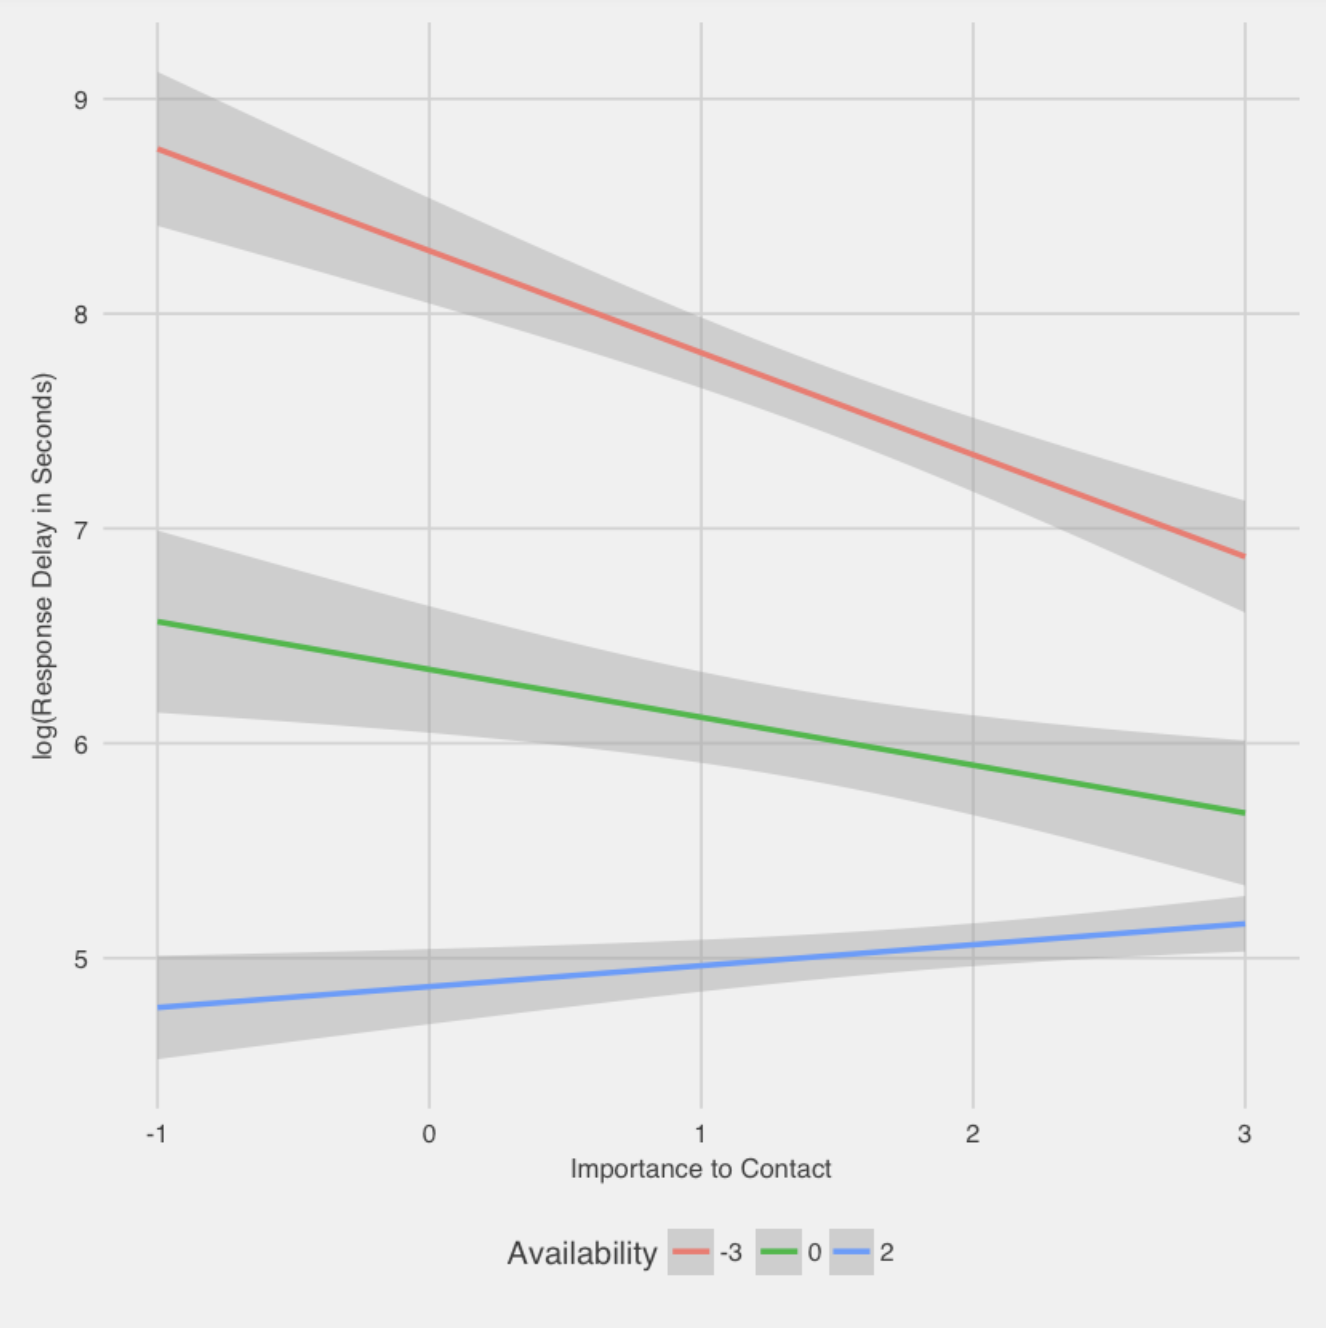
\includegraphics[width=.7\textwidth]{figures/importance_contact_availability_interaction}
\caption{Distribution of response time in seconds.}
\label{fig:importance_contact_availability_interaction}
\end{figure}

\begin{figure}[h]
\centering
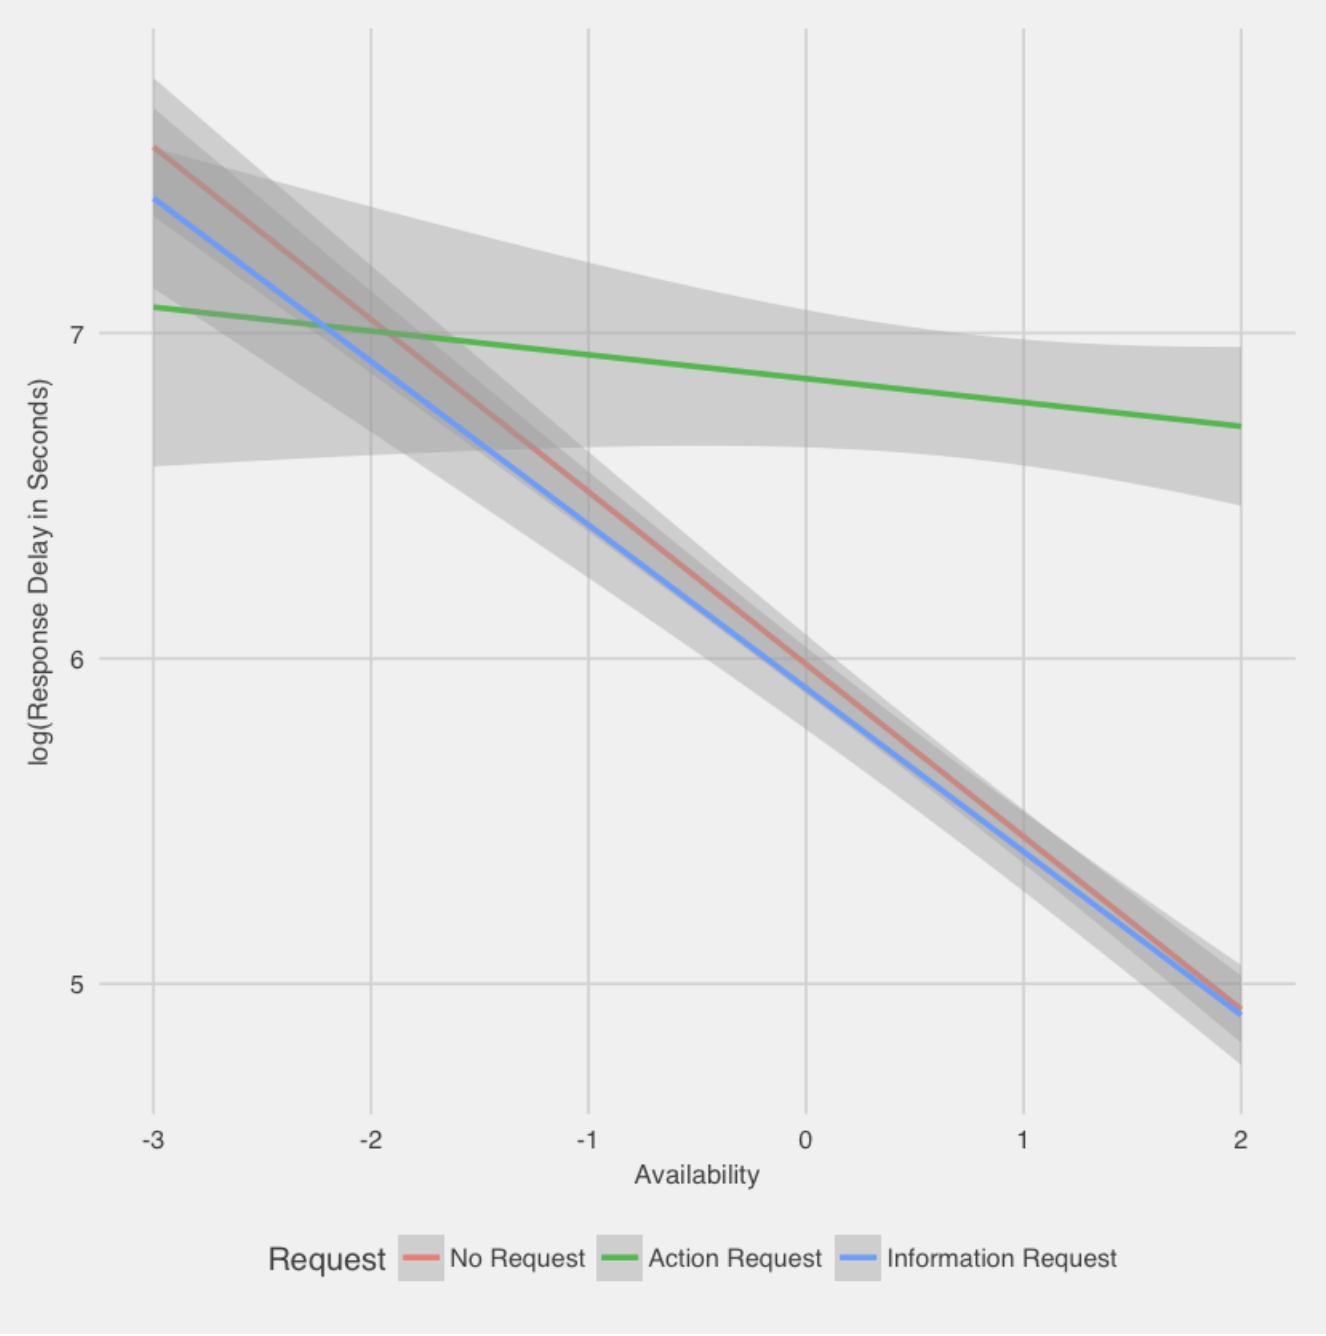
\includegraphics[width=.7\textwidth]{figures/request_availability_interaction}
\caption{Distribution of response time in seconds.}
\label{fig:request_availability_interaction}
\end{figure}


\chapter{Discussion}

 \renewcommand\refname{\begin{centering}References\end{centering}}
 \bibliography{references.bib}
 \bibliographystyle{apacite} %or another suitable style.



% \appendix		% Appendix begins here (optional).

%\appendices	        % If more than one appendix chapters,
				% use appendices instead of appendix




\end{document}

